\begin{chapterpage}{Introduction to data}
  \chaptertitle{Introduction to data}
  \label{introductionToData}
  \label{ch_intro_to_data}
  \chaptersection{basicExampleOfStentsAndStrokes}
  \chaptersection{dataBasics}
  \chaptersection{overviewOfDataCollectionPrinciples}
  % \chaptersection{section_obs_data_sampling}
  \chaptersection{experimentsSection}
\end{chapterpage}
\renewcommand{\chapterfolder}{ch_intro_to_data}

%\begin{tipBox}{\tipBoxTitle[Chapter Goal:]{Thinking about data}
%Understand basics about data organization, data types, numerical summaries of data, graphical summaries of data, and foundational techniques for data collection. We begin and end the chapter with case studies.}
%\end{tipBox}

\chapterintro{Scientists seek to answer questions
  using rigorous methods and careful observations.
  These observations -- collected from the likes of field notes,
  surveys, and experiments -- form the backbone of a statistical
  investigation and are called \term{data}.
  Statistics is the study of how best to collect, analyze,
  and draw conclusions from data, %It is helpful to put statistics in the context of a general process of investigation:
%\begin{enumerate}
%\setlength{\itemsep}{0mm}
%\item Identify a question or problem.
%\item Collect relevant data on the topic.
%\item Analyze the data.
%\item Form a conclusion.
%%\item Make decisions based on the conclusion.
%\end{enumerate}
%Statistics as a subject focuses on making stages 2-4 objective, rigorous, and efficient. That~is, statistics has three primary components: How best can we collect data? How should it be analyzed? And what can we infer from the analysis?
  and in this first chapter,
  we focus on both the properties of data
  and on the collection of data.}

%The topics scientists investigate are as diverse as the questions they ask. However, many of these investigations can be addressed with a small number of data collection techniques, analytic tools, and fundamental concepts in statistical inference. This chapter provides a glimpse into these and other themes we will encounter throughout the rest of the book. We introduce the basic principles of each branch and learn some tools along the way. We will encounter applications from other fields, some of which are not typically associated with science but nonetheless can benefit from statistical study.



\section{Case study: using stents to prevent strokes}
\label{basicExampleOfStentsAndStrokes}

\index{data!stroke|(}

Section~\ref{basicExampleOfStentsAndStrokes} introduces a classic challenge in statistics: evaluating the efficacy of a medical treatment. Terms in this section, and indeed much of this chapter, will all be revisited later in the text. The plan for now is simply to get a sense of the role statistics can play in practice.

In this section we will consider an experiment that studies effectiveness of stents in treating patients at risk of stroke.
Stents are devices put inside blood vessels that assist in patient recovery after cardiac events and reduce the risk of an additional heart attack or death. Many doctors have hoped that there would be similar benefits for patients at risk of stroke. We start by writing the principal question the researchers hope to answer:
\begin{quote}
Does the use of stents reduce the risk of stroke?
\end{quote}

The researchers who asked this question conducted an experiment with 451 at-risk patients. Each volunteer patient was randomly assigned to one of two groups:
\begin{itemize}
\item[]\termsub{Treatment group}{treatment group}. Patients in the treatment group received a stent and medical management. The medical management included medications, management of risk factors, and help in lifestyle modification.
\item[]\termsub{Control group}{control group}. Patients in the control group received the same medical management as the treatment group, but they did not receive stents.
\end{itemize}
Researchers randomly assigned 224 patients to the treatment group and 227 to the control group. In this study, the control group provides a reference point against which we can measure the medical impact of stents in the treatment group.

Researchers studied the effect of stents at two time points: 30~days after enrollment and 365~days after enrollment. The results of 5 patients are summarized in Figure~\ref{stentStudyResultsDF}. Patient outcomes are recorded as ``stroke'' or ``no event'', representing whether or not the patient had a stroke at the end of a time period.

\begin{figure}[h]
\centering
\begin{tabular}{l ccc}
\hline
Patient	&	group	&	0-30 days 	&	0-365 days \\
\hline
1		&	treatment &	no event &	no event \\
2		&	treatment &	stroke & stroke \\
3		&	treatment &	no event & no event \\
$\vdots$	&	$\vdots$	  &	$\vdots$ \\
450	&	control &	no event &	no event \\
451	&	control &	no event &	no event \\
\hline
\end{tabular}
\caption{Results for five patients from the stent study.}
\label{stentStudyResultsDF}
% trmt <- c(rep('trmt', 224), rep('control', 227)); outcome30 <- c(rep(c('event', 'no_event'), c(33, 191)), rep(c('event', 'no_event'), c(13, 214))); outcome365 <- c(rep(c('event', 'no_event'), c(33, 191)), rep(c('event', 'no_event'), c(13, 214)))
\end{figure}

Considering data from each patient individually would be a long, cumbersome path towards answering the original research question. Instead, performing a statistical data analysis allows us to consider all of the data at once. Figure~\ref{stentStudyResults} summarizes the raw data in a more helpful way. In this table, we can quickly see what happened over the entire study. For instance, to identify the number of patients in the treatment group who had a stroke within 30 days, we look on the left-side of the table at the intersection of the treatment and stroke: 33.

\begin{figure}[h]
\centering
\begin{tabular}{l cc c cc}
& \multicolumn{2}{c}{0-30 days} &\hspace{5mm}\ & \multicolumn{2}{c}{0-365 days} \\
  \cline{2-3} \cline{5-6}
	& 	stroke 	& no event && 	stroke 	& no event \\
  \hline
treatment 	& 33		& 191	&&	45 	& 179 \\
control 		& 13		& 214	&& 	28	& 199 \\
  \hline
Total				& 46		& 405	&&	73	& 378 \\
  \hline
\end{tabular}
\caption{Descriptive statistics for the stent study.}
\label{stentStudyResults}
\end{figure}

\begin{exercisewrap}
\begin{nexercise}
Of the 224 patients in the treatment group, 45 had a stroke by the end of the first year. Using these two numbers, compute the proportion of patients in the treatment group who had a stroke by the end of their first year. (Please note: answers to all Guided Practice exercises are provided using footnotes.)\footnotemark
\end{nexercise}
\end{exercisewrap}\footnotetext{The proportion of the 224 patients who had a stroke within 365 days: $45/224 = 0.20$.}

We can compute summary statistics from the table.
A \term{summary statistic}%
\index{statistic|seealso{summary statistic}}
is a single number summarizing
a large amount of data.
For instance, the primary results of the study after 1~year
could be described by two summary statistics:
the proportion of people who had a stroke in the treatment
and control groups.
\begin{itemize}
\setlength{\itemsep}{0mm}
\item[] Proportion who had a stroke in the treatment (stent) group: $45/224 = 0.20 = 20\%$.
\item[] Proportion who had a stroke in the control group: $28/227 = 0.12 = 12\%$.
\end{itemize}
These two summary statistics are useful in looking for differences in the groups, and we are in for a surprise: an additional 8\% of patients in the treatment group had a stroke! This is important for two reasons. First, it is contrary to what doctors expected, which was that stents would \emph{reduce} the rate of strokes. Second, it leads to a statistical question: do the data show a ``real'' difference between the groups?

This second question is subtle. Suppose you flip a coin 100 times. While the chance a coin lands heads in any given coin flip is 50\%, we probably won't observe exactly 50 heads. This type of fluctuation is part of almost any type of data generating process. It is possible that the 8\% difference in the stent study is due to this natural variation. However, the larger the difference we observe (for a particular sample size), the less believable it is that the difference is due to chance. So what we are really asking is the following: is the difference so large that we should reject the notion that it was due to chance?

While we don't yet have our statistical tools to fully address this question on our own, we can comprehend the conclusions of the published analysis: there was compelling evidence of harm by stents in this study of stroke patients.

\textbf{Be careful:}
Do not generalize the results of this study to all patients
and all stents.
This study looked at patients with very specific characteristics
who volunteered to be a part of this study and who may not be
representative of all stroke patients.
In addition, there are many types of stents and this study only
considered the self-expanding Wingspan stent (Boston Scientific).
However, this study does leave us with an important lesson:
we should keep our eyes open for surprises.

\index{data!stroke|)}


{\exercisesheader{}

% 1

\eoce{\qt{Migraine and acupuncture,
    Part 1\label{migraine_and_acupuncture_intro}}
A migraine is a particularly painful type of headache,
which patients sometimes wish to treat with acupuncture.
To determine whether acupuncture relieves migraine 
pain, researchers conducted a randomized controlled study
where 89 females diagnosed with migraine headaches were
randomly assigned to one of two groups:
treatment or control.
43 patients in the treatment group received acupuncture 
that is specifically designed to treat migraines.
46 patients in the control group received placebo acupuncture
(needle insertion at non-acupoint locations).
24 hours after patients received acupuncture, they were asked 
if they were pain free.
Results are summarized in the contingency table
below.\footfullcite{Allais:2011}

\noindent\begin{minipage}[l]{0.4\textwidth}
\begin{tabular}{ll  cc c} 
			                         		&           & \multicolumn{2}{c}{\textit{Pain free}} \\
\cline{3-4}
			                        	 	&			& Yes 	& No 	                  & Total \\
\cline{2-5}
							& Treatment 	& 10	 	& 33		                  & 43 \\
\raisebox{1.5ex}[0pt]{\emph{Group}} & Control	 	& 2	 	& 44 	 	                  & 46 \\
\cline{2-5}
							& Total		& 12		& 77		                  & 89
\end{tabular}
\end{minipage}
\begin{minipage}[c]{0.05\textwidth}
\end{minipage}
\begin{minipage}[c]{0.27\textwidth}
\begin{center}
\includegraphics[width = 0.75\textwidth]{ch_intro_to_data/figures/eoce/migraine_and_acupuncture_intro/earacupuncture.pdf}
\end{center}
\end{minipage}
\begin{minipage}[c]{0.25\textwidth}
{\footnotesize Figure from the original paper displaying the appropriate area 
(M) versus the inappropriate area (S) used in the treatment of migraine attacks.}
\end{minipage}
\begin{parts}
\item What percent of patients in the treatment group were pain free 24 hours 
after receiving acupuncture? 
\item What percent were pain free in the control group?
\item In which group did a higher percent of patients become pain free 24 hours 
after receiving acupuncture?
\item Your findings so far might suggest that acupuncture is an effective treatment 
for migraines for all people who suffer from migraines. However this is not the 
only possible conclusion that can be drawn based on your findings so far. What is 
one other possible explanation for the observed difference between the percentages 
of patients that are pain free 24 hours after receiving acupuncture in the two groups?
\end{parts}
}{}

% 2

\eoce{\qt{Sinusitis and antibiotics,
    Part 1\label{sinusitis_and_antibiotics_intro}} 
Researchers studying the effect of antibiotic treatment for acute sinusitis 
compared to symptomatic treatments randomly assigned 166 adults diagnosed 
with acute sinusitis to one of two groups: treatment or control. Study 
participants received either a 10-day course of amoxicillin (an antibiotic) 
or a placebo similar in appearance and taste. The placebo consisted of 
symptomatic treatments such as acetaminophen, nasal decongestants, etc.
At the end of the 10-day period, patients were asked if
they experienced improvement in symptoms.
The distribution of responses is summarized below. 
\footfullcite{Garbutt:2012}
\begin{center}
\begin{tabular}{ll  cc c} 
                                    			&			& \multicolumn{2}{c}{\textit{Self-reported improvement}} \\
                                    			&			& \multicolumn{2}{c}{\textit{in symptoms}} \\
\cline{3-4}
			                        		&			& Yes 	& No 	& Total \\
\cline{2-5}
							& Treatment 	& 66		& 19		& 85 \\
\raisebox{1.5ex}[0pt]{\emph{Group}}	& Control		& 65		& 16 		& 81 \\
\cline{2-5}
							& Total		& 131	& 35		& 166
\end{tabular}
\end{center}
\begin{parts}
\item What percent of patients in the treatment group experienced improvement 
in symptoms? 
\item What percent experienced improvement in symptoms in the 
control group?
\item In which group did a higher percentage of patients experience improvement
in symptoms?
\item Your findings so far might suggest that a real difference in effectiveness of 
antibiotic and placebo treatments for improving symptoms of sinusitis. However this is 
not the only possible conclusion that can be drawn based on your findings so far. What is 
one other possible explanation for the observed difference between the percentages 
of patients that are pain free 24 hours after receiving acupuncture in the two groups?
\end{parts}
}{}
}



\section{Data basics}
\label{dataBasics}

Effective organization and description of data is a first
step in most analyses.
This section introduces the \emph{data matrix} for organizing
data as well as some terminology about different forms of data
that will be used throughout this book.

\subsection{Observations, variables, and data matrices}

\index{data!loan50|(}

Figure~\ref{loan50DF} displays rows 1, 2, 3, and 50 of a data set
for 50 randomly sampled loans offered through Lending Club,
which is a peer-to-peer lending company.
These observations will be referred to as the
\data{loan50} data set.

Each row in the table represents a single loan.
The formal name for a row is a \term{case}
or \term{observational unit}\index{unit of observation}.
The columns represent characteristics,
called \termsub{variables}{variable},
for each of the loans.
For example, the first row represents a loan of \$7,500 with an interest rate of 7.34\%, where the borrower is based in Maryland (MD) and has an income of \$70,000.

\begin{exercisewrap}
\begin{nexercise}
What is the grade of the first loan in Figure~\ref{loan50DF}?
And what is the home ownership status of the borrower
for that first loan?
For these Guided Practice questions, you can check your answer
in the footnote.\footnotemark{}
\end{nexercise}
\end{exercisewrap}
\footnotetext{The loan's grade is A,
  and the borrower rents their residence.}

In practice, it is especially important to ask clarifying
questions to ensure important aspects of the data are understood.
For instance, it is always important to be sure we know what
each variable means and the units of measurement.
Descriptions of the \data{loan50} variables are given
in Figure~\ref{loan50Variables}.

\begin{figure}[h]
\centering
{\small
\begin{tabular}{ccc ccc cc} %c}
  \hline
   & \var{loan\us{}amount}
   & \var{interest\us{}rate}
   & \var{term} & \var{grade} & \var{state}
   & \var{total\us{}income}
   & \var{homeownership} \\
  \hline
  1 & 7500 & 7.34 & 36 & A & MD & 70000 & rent \\
  2 & 25000 & 9.43 & 60 & B & OH & 254000 & mortgage \\
  3 & 14500 & 6.08 & 36 & A & MO & 80000 & mortgage \\
  $\vdots$ & $\vdots$ & $\vdots$ & $\vdots$ & $\vdots$ & $\vdots$
      & $\vdots$ & $\vdots$ \\
  50 & 3000 & 7.96 & 36 & A & CA & 34000 & rent \\
   \hline
\end{tabular}
}
\caption{Four rows from the \data{loan50} data matrix.}
\label{loan50DF}
\end{figure}
% Dropped: state, verified_income
% library(openintro); vars <- c("loan_amount", "interest_rate", "term", "grade", "total_income", "home_ownership", "loan_status"); library(xtable); data(loan50); loan50[c(1,2,3,50), vars]; xtable(loan50[c(1,2,3,50), vars])

\begin{figure}[h]
\centering\small
\begin{tabular}{lp{10.5cm}}
\hline
{\bf variable} & {\bf description} \\
\hline
\var{loan\us{}amount} & Amount of the loan received,
    in US dollars.  \\
\var{interest\us{}rate} & Interest rate on the loan,
    in an annual percentage.  \\
\var{term} & The length of the loan, which is always set
    as a whole number of months. \\
\var{grade} & Loan grade, which takes a values A through G
    and represents the quality of the loan and its likelihood
    of being repaid.  \\
\var{state} & US state where the borrower resides. \\
\var{total\us{}income} & Borrower's total income,
    including any second income, in US dollars.   \\
\var{homeownership} & Indicates whether the
    person owns, owns but has a mortgage, or rents.  \\
%\var{verified\us{}income} & Indicates whether the
%    income is verified, its source is verified but not the amount,
%    or it is not verified.   \\
\hline
\end{tabular}
\caption{Variables and their descriptions for the \data{loan50} data set.}
\label{loan50Variables}
\end{figure}

\index{data!loan50|)}

The data in Figure~\ref{loan50DF} represent a \term{data matrix},
which is a convenient and common way to organize data,
especially if collecting data in a spreadsheet.
Each row of a data matrix corresponds to a unique case
(observational unit),
and each column corresponds to a variable.
%A data matrix for the stroke study introduced in
%Section~\ref{basicExampleOfStentsAndStrokes} is shown
%in Figure~\vref{stentStudyResultsDF}, where the cases were
%patients and three variables were recorded for each
%patient.

\D{\newpage}

When recording data, use a data matrix unless you have
a very good reason to use a different structure.
This structure allows new cases to be added as rows
or new variables as new columns.

\begin{exercisewrap}
\begin{nexercise}
The grades for assignments, quizzes, and exams in a course are
often recorded in a gradebook that takes the form of a data matrix.
How might you organize grade data using a data
matrix?\footnotemark
\end{nexercise}
\end{exercisewrap}

\index{data!county|(}

\begin{exercisewrap}
\begin{nexercise}\label{desc_county_as_data_matrix}%
We consider data for 3,142 counties in the United States,
which includes each county's name,
the state where it resides, its population in 2017,
how its population changed from 2010 to 2017,
poverty rate,
and six additional characteristics.
How might these data be organized in
a data matrix?\footnotemark
\end{nexercise}
\end{exercisewrap}
\addtocounter{footnote}{-1}
\footnotetext{There are multiple strategies that can be followed.
  One common strategy is to have each student represented by a row,
  and then add a column for each assignment, quiz, or exam.
  Under this setup, it is easy to review a single line to understand
  a student's grade history.
  There should also be columns to include student information,
  such as one column to list student names.}
\addtocounter{footnote}{1}
\footnotetext{Each county may be viewed as a case,
  and there are eleven pieces of information recorded for
  each case.
  A table with 3,142 rows and 11 columns could hold these data,
  where each row represents a county and each column represents
  a particular piece of information.}

The data described in Guided
Practice~\ref{desc_county_as_data_matrix} represents the
\data{county} data set, which is shown as a data matrix
in Figure~\ref{countyDF}.
The variables are summarized in Figure~\ref{countyVariables}.

\begin{landscape}
\begin{figure}
\centering\small
\begin{tabular}{ccc ccc ccc ccc}
  \hline
 & \var{name} & \var{state} & \var{pop} & \var{pop\us{}change} & \var{poverty} & \var{homeownership} & \var{multi\us{}unit} & \var{unemp\us{}rate} & \var{metro} & \var{median\us{}edu} & \var{median\us{}hh\us{}income} \\ 
  \hline
1 & Autauga  & Alabama &  55504 &  1.48 & 13.7 & 77.5 &  7.2 & 3.86 & yes & some\us{}college & 55317 \\ 
  2 & Baldwin  & Alabama & 212628 &  9.19 & 11.8 & 76.7 & 22.6 & 3.99 & yes & some\us{}college & 52562 \\ 
  3 & Barbour  & Alabama &  25270 & -6.22 & 27.2 & 68.0 & 11.1 & 5.90 & no  & hs\us{}diploma   & 33368 \\ 
  4 & Bibb     & Alabama &  22668 &  0.73 & 15.2 & 82.9 &  6.6 & 4.39 & yes & hs\us{}diploma   & 43404 \\ 
  5 & Blount   & Alabama &  58013 &  0.68 & 15.6 & 82.0 &  3.7 & 4.02 & yes & hs\us{}diploma   & 47412 \\ 
  6 & Bullock  & Alabama &  10309 & -2.28 & 28.5 & 76.9 &  9.9 & 4.93 & no  & hs\us{}diploma   & 29655 \\ 
  7 & Butler   & Alabama &  19825 & -2.69 & 24.4 & 69.0 & 13.7 & 5.49 & no  & hs\us{}diploma   & 36326 \\ 
  8 & Calhoun  & Alabama & 114728 & -1.51 & 18.6 & 70.7 & 14.3 & 4.93 & yes & some\us{}college & 43686 \\ 
  9 & Chambers & Alabama &  33713 & -1.20 & 18.8 & 71.4 &  8.7 & 4.08 & no  & hs\us{}diploma   & 37342 \\ 
  10 & Cherokee & Alabama &  25857 & -0.60 & 16.1 & 77.5 &  4.3 & 4.05 & no  & hs\us{}diploma   & 40041 \\ 
  $\vdots$ & $\vdots$ & $\vdots$ & $\vdots$ & $\vdots$ & $\vdots$ & $\vdots$ & $\vdots$ & $\vdots$ & $\vdots$ & $\vdots$ & $\vdots$ \\
  3142 & Weston   & Wyoming &   6927 & -2.93 & 14.4 & 77.9 &  6.5 & 3.98 & no  & some\us{}college & 59605 \\ 
   \hline
\end{tabular}
\caption{Eleven rows from the \data{county} data set.}
\label{countyDF}
% library(openintro); data(county); county$name <- gsub(" County$", "", county$name); county$pop <- county$pop2017; county$unemp_rate = county$unemployment_rate; these <- c("name", "state", "pop", "pop_change", "poverty", "homeownership", "multi_unit", "unemp_rate", "metro", "median_edu", "median_hh_income"); county <- county[, these]; library(xtable); xtable(as.data.frame(lapply(rbind.data.frame(head(county, 10), tail(county, 1)), function(x) { format(x) })))
\end{figure}

\begin{figure}
\centering\small
\begin{tabular}{lp{11cm}}
\hline
{\bf variable} & {\bf description} \\
\hline
\var{name} &
    County name. \\
\var{state} &
    State where the county resides,
    or the District of Columbia. \\
\var{pop} &
    Population in 2017. \\
\var{pop\us{}change} &
    Percent change in the population from 2010 to 2017.
    For example, the value \resp{1.48} in the first row
    means the population for this county
    increased by 1.48\% from 2010 to 2017. \\
\var{poverty} &
    Percent of the population in poverty. \\
\var{homeownership}  &
    Percent of the population that lives in their own home
    or lives with the owner, e.g. children living with parents
    who own the home. \\
\var{multi\us{}unit}  &
    Percent of living units that are in multi-unit structures,
    e.g. apartments. \\
\var{unemp\us{}rate} &
    Unemployment rate as a percent. \\
\var{metro} &
    Whether the county contains a metropolitan area. \\
\var{median\us{}edu} & Median education level, which
    can take a value among
    \resp{below\us{}hs},
    \resp{hs\us{}diploma},
    \resp{some\us{}college},
    and \resp{bachelors}. \\
\var{median\us{}hh\us{}income} &
    Median household income for the county, where a household's
    income equals the total income of its occupants who are
    15~years or older. \\
%\var{per\us{}capita\us{}income} &
%    Per capita (per person) income for the county. \\
\hline
\end{tabular}
\centering
\caption{Variables and their descriptions for the \data{county} data set.}
\label{countyVariables}
\end{figure}
\end{landscape}

\subsection{Types of variables}
\label{variableTypes}

Examine the \var{unemp\us{}rate}, \var{pop}, \var{state},
and \var{median\us{}edu} variables in the \data{county}
data set. Each of these variables is inherently different from the
other three, yet some share certain characteristics.

First consider \var{unemp\us{}rate},
which is said to be a \term{numerical} variable since
it can take a wide range of numerical values,
and it is sensible to add, subtract, or take averages
with those values.
On the other hand, we would not classify a variable
reporting telephone area codes as numerical since the
average, sum, and difference of area codes doesn't have
any clear meaning.

The \var{pop} variable is also numerical, although it seems
to be a little different than \var{unemp\us{}rate}.
This variable of the population count can only take whole
non-negative numbers (\resp{0}, \resp{1}, \resp{2}, ...).
For~this reason, the population variable is said to be
\term{discrete} since it can only take numerical values
with jumps.
On the other hand, the unemployment rate variable is said
to be \term{continuous}.

The variable \var{state} can take up to 51 values after
accounting for Washington, DC: \resp{AL}, \resp{AK}, ...,
and \resp{WY}.
Because the responses themselves are categories,
\var{state} is called a \term{categorical} variable,
and the possible values are called the variable's \term{levels}.

Finally, consider the \var{median\us{}edu} variable,
which describes the median education level of county
residents and takes values
\resp{below\us{}hs}, \resp{hs\us{}diploma},
\resp{some\us{}college}, or \resp{bachelors}
in each county.
This variable seems to be a hybrid: it is a categorical variable
but the levels have a natural ordering.
A variable with these properties is called an \term{ordinal}
variable, while a regular categorical variable without this
type of special ordering is called a \term{nominal} variable.
To simplify analyses, any ordinal variable in this book will
be treated as a nominal (unordered) categorical variable.

\begin{figure}[h]
  \centering
  \Figure{0.57}{variables}
  \caption{Breakdown of variables into their respective types.}
  \label{variables}
\end{figure}

\begin{examplewrap}
\begin{nexample}{Data were collected about students
    in a statistics course.
    Three variables were recorded for each student:
    number of siblings, student height, and whether
    the student had previously taken a statistics course.
    Classify each of the variables as continuous numerical,
    discrete numerical, or categorical.}
  The number of siblings and student height represent
  numerical variables.
  Because the number of siblings is a count, it is discrete.
  Height varies continuously, so it is a continuous numerical
  variable.
  The last variable classifies students into two categories
  -- those who have and those who have not taken a statistics
  course -- which makes this variable categorical.
\end{nexample}
\end{examplewrap}

\begin{exercisewrap}
\begin{nexercise}\index{data!stroke}%
An experiment is evaluating the effectiveness of a new drug
in treating migraines.
A \var{group} variable is used to indicate the experiment group
for each patient: treatment or control.
The \mbox{\var{num\us{}migraines}} variable represents the number
of migraines the patient experienced during a 3-month period.
\mbox{Classify} each variable as either numerical or
categorical?\footnotemark
\end{nexercise}
\end{exercisewrap}
\footnotetext{There
  \var{group} variable can take just one of two group names,
  making it categorical.
  The \var{num\us{}migraines} variable describes
  a count of the number of migraines, which is an outcome where
  basic arithmetic is sensible, which means this is numerical
  outcome; more specifically, since it represents a count,
  \var{num\us{}migraines} is a discrete numerical variable.}


\D{\newpage}

\subsection{Relationships between variables}
\label{variableRelations}

Many analyses are motivated by a researcher looking
for a relationship between two or more variables.
A social scientist may like to answer some of the
following questions:
\newcommand{\popchangevmedianhhincomequestion}[0]{
    % Note that this question is used to introduce the
    %explanatory / response variable topic.
    Does a higher than average increase in county population
    tend to correspond to counties with higher or lower median
    household incomes?}%
\begin{enumerate}
\setlength{\itemsep}{0mm}
\item[(1)]\label{ownershipMultiUnitQuestion}
    If homeownership is lower than the national average
    in one county, will the percent of multi-unit structures
    in that county tend to be above or below the national average?
\item[(2)]\label{pop_change_v_median_hh_income_question}
    \popchangevmedianhhincomequestion{}
    % Do counties with a higher median household income
    % tend to be growing faster or slower than other counties?
\item[(3)]\label{isAverageIncomeAssociatedWithSmokingBans}
    How useful a predictor is median education level
    for the median household income for US counties?
\end{enumerate}

To answer these questions, data must be collected, such
as the \data{county} data set shown in Figure~\ref{countyDF}.
Examining summary statistics \index{summary statistic} could
provide insights for each of the three questions about counties.
Additionally, graphs can be used to visually explore data.

\indexthis{Scatterplots}{scatterplot} are one type of graph
used to study the relationship between two numerical variables.
Figure~\ref{multiunitsVsOwnership} compares the variables
\var{homeownership} and
\var{multi\us{}unit},
which is the percent of units in multi-unit structures
(e.g. apartments, condos).
Each point on the plot represents a single county.
For instance, the highlighted dot corresponds to
County~413 in the \data{county} data set:
Chattahoochee County, Georgia, which has 39.4\% of
units in multi-unit structures and a homeownership rate
of 31.3\%.
The scatterplot suggests a relationship between the
two variables: counties with a higher rate of multi-units
tend to have lower homeownership rates.
We might brainstorm as to why this relationship exists
and investigate each idea to determine which are the most
reasonable explanations.

\begin{figure}[h]
  \centering
  \Figure{0.79}{multiunitsVsOwnership}
  \caption{A scatterplot of homeownership versus the percent
      of units that are in multi-unit structures for US counties.
      The highlighted dot represents Chattahoochee County, Georgia,
      which has a multi-unit rate of 39.4\% and a homeownership rate
      of 31.3\%.}
  \label{multiunitsVsOwnership}
\end{figure}

The multi-unit and homeownership rates are said to be
associated because the plot shows a discernible pattern.
When two variables show some connection with one another,
they are called \term{associated} variables.
Associated variables can also be called \term{dependent}
variables and vice-versa.

\D{\newpage}

\begin{exercisewrap}
\begin{nexercise}
Examine the variables in the \data{loan50} data set,
which are described in Figure~\vref{loan50Variables}.
Create two questions about possible relationships
between variables in \data{loan50} that are of interest
to~you.\footnotemark
\end{nexercise}
\end{exercisewrap}
\footnotetext{Two example questions:
  (1)~What is the relationship between loan amount and
      total income?
  (2)~If someone's income is above the average, will their
      interest rate tend to be above or below the average?}

\begin{examplewrap}
\begin{nexample}{This example examines the relationship
    between a county's population change
    from 2010 to 2017
    and median household income,
    which is visualized as a scatterplot in
    Figure~\ref{pop_change_v_med_income}.
    Are these variables associated?}
  The larger the median household income for a county,
  the higher the population growth observed for the county.
  While this trend isn't true for every county,
  the trend in the plot is evident.
  Since there is some relationship between the variables,
  they are associated.
\end{nexample}
\end{examplewrap}

%When two variables show some connection with one another,
%they are called \term{associated} variables.
%Associated variables can also be called \term{dependent}
%variables and vice-versa.
%When the variables increase together,
%as they do in Figure~\ref{loan_amount_vs_income},
%they are said to be \term{positively associated}.
%When the trend in the scatterplot goes down to the right,
%then they are described as \term{negatively correlated}.

%While we may find it interesting to consider the relationship
%between two variables such as those in the scatterplot,
%the relationship between those variables can be more complex.
%For example, interest rates on loans tend to be chosen based
%on the riskiness of the loan, i.e. how likely it is to be
%paid back, and that is likely to depend on a variety of
%details, such as what the loan is for, the person's
%creditworthiness, whether their income is verified, etc.
%We will begin exploring some of these more complex relationships
%in graphs in Chapter~\ref{ch_summarizing_data} and beyond.
%\Comment{Revise if we don't add these more rich plots...}

%\begin{example}{Figure~\ref{interest_rate_vs_loan_amount}
%    features a scatterplot of interest rate against loan amount.
%    Are these variables associated?}
%  There isn't an evident trend in the data,
%  so we would say these two variables are not associated.
%\end{example}

\begin{figure}
  \centering
  \Figure{0.9}{pop_change_v_med_income}
  \caption{A scatterplot showing
      \var{pop\us{}change}
      against \var{median\us{}hh\us{}income}.
      Owsley County of Kentucky, is highlighted,
      which lost 3.63\% of its population from 2010 to 2017
      and had median household income of \$22,736.}
  \label{pop_change_v_med_income}
\end{figure}

Because there is a downward trend in
Figure~\ref{multiunitsVsOwnership} --
counties with more units in multi-unit structures
are associated with lower homeownership --
these variables are said to be
\termsub{negatively associated}{negative association}.
A~\term{positive association} is shown in the relationship
between the
\var{median\us{}hh\us{}income}
and \var{pop\us{}change}
in Figure~\ref{pop_change_v_med_income},
where counties with higher median household income tend
to have higher rates of population growth.

If two variables are not associated,
then they are said to be \term{independent}.
That is, two variables are independent if there
is no evident relationship between the two.

\begin{onebox}{Associated or independent, not both}
A pair of variables are either related in some way (associated) or not (independent). No pair of variables is both associated and independent.
\end{onebox}


\D{\newpage}

\subsection{Explanatory and response variables}
\label{explanatoryAndResponse}

When we ask questions about the relationship
between two variables, we sometimes also want to determine
if the change in one variable causes a change in the other.
Consider the following rephrasing of an earlier question
about the \data{county} data set:
\begin{quote}\em
  If there is an increase in the median household income
  in a county, does this drive an increase in its population?
\end{quote}
In this question, we are asking whether one variable
affects another.
If this is our underlying belief,
then \emph{median household income} is the
\termsub{explanatory}{explanatory variable}
variable and the \emph{population change} is the
\termsub{response}{response variable} variable
in the hypothesized relationship.\footnote{Sometimes
  the explanatory variable is called the \term{independent}
  variable and the response variable is called the
  \term{dependent} variable.
  However, this becomes confusing since a \emph{pair}
  of variables might be independent or dependent,
  so we avoid this language.}

\index{data!county|)}

\begin{onebox}{Explanatory and response variables}
When we suspect one variable might causally affect another,
we label the first variable the explanatory variable and the
second the response variable.
\vspace{1mm}

\hspace{10mm}\includegraphics[height=0.34in]{ch_intro_to_data/figures/expResp/expResp}

For many pairs of variables, there is no hypothesized
relationship, and these labels would not be applied to
either variable in such cases.
\end{onebox}

Bear in mind that the act of labeling the variables in this
way does nothing to guarantee that a causal relationship exists.
A formal evaluation to check whether one variable causes
a change in another requires an experiment.

%\begin{exercisewrap}
%\begin{nexercise}
%Consider the earlier question:
%\begin{quote}\em
%  If a county has a higher median household income,
%  does this drive an increase in its population?
%\end{quote}
%We could have just as easily reframed the causal relationship
%to be in the reverse direction:
%\begin{quote}\em
%  If a county more population growth, does this drive
%  it to have a higher median household income?
%\end{quote}
%What are the explanatory and response variables when framing
%the variable relationship in the second question?
%\end{nexercise}
%\end{exercisewrap}
%\footnotetext{In this framing, we have hypothesized
%  that population growth drives median household income.
%  That is, population growth is the explanatory variable,
%  and median household income is the response.
%  This exercise should emphasize that these variable labels
%  do not actually define whether one variable actually affects
%  the other.}


\subsection{Introducing observational studies and experiments}

\noindent%
There are two primary types of data collection:
observational studies and experiments.

Researchers perform an \term{observational study} when they
collect data in a way that does not directly interfere with
how the data arise.
For instance, researchers may collect information via surveys,
review medical or company records, or follow a \term{cohort}
of many similar individuals to form hypotheses about why certain
diseases might develop.
In each of these situations, researchers merely observe the
data that arise.
In general, observational studies can provide evidence of
a naturally occurring association between variables, but they
cannot by themselves show a causal connection.

When researchers want to investigate the possibility of
a causal connection, they conduct an \term{experiment}.
Usually there will be both an explanatory and a response
variable.
For instance, we may suspect administering a drug will reduce
mortality in heart attack patients over the following year.
To check if there really is a causal connection between the
explanatory variable and the response, researchers will collect
a sample of individuals and split them into groups.
The individuals in each group are \emph{assigned} a treatment.
When individuals are randomly assigned to a group,
the experiment is called a \term{randomized experiment}.
For example, each heart attack patient in the drug trial
could be randomly assigned,  perhaps by flipping a coin,
into one of two groups:
the first group receives a \term{placebo} (fake treatment)
and the second group receives the drug.
See the case study in
Section~\ref{basicExampleOfStentsAndStrokes} for another
example of an experiment, though that study did not employ
a~placebo.

\begin{onebox}{Association $\neq$ Causation}
  In general, association does not imply causation,
  and causation can only be inferred from a randomized experiment.
\end{onebox}


{\exercisesheader{}

% 3

\eoce{\qt{Air pollution and birth outcomes, study components\label{study_components_airpoll}} 
Researchers collected data to examine the relationship between air pollutants 
and preterm births in Southern California. During the study air pollution levels 
were measured by air quality monitoring stations. Specifically, levels of carbon 
monoxide were recorded in parts per million, nitrogen dioxide and ozone in parts 
per hundred million, and coarse particulate matter (PM$_{10}$) in $\mu g/m^3$. 
Length of gestation data were collected on 143,196 births between the years 1989 
and 1993, and air pollution exposure during gestation was calculated for each 
birth. The analysis suggested that increased ambient PM$_{10}$ and, to a lesser 
degree, CO concentrations may be associated with the occurrence of preterm births.\footfullcite{Ritz+Yu+Chapa+Fruin:2000}
\begin{parts}
\item Identify the main research question of the study.
\item Who are the subjects in this study, and how many are included?
\item What are the variables in the study? Identify each variable as numerical or 
categorical. If numerical, state whether the variable is discrete or continuous.
If categorical, state whether the variable is ordinal.
\end{parts}
}{}

% 4

\eoce{\qt{Buteyko method, study components\label{study_components_buteyko}} 
The Buteyko method is a shallow breathing technique developed by Konstantin 
Buteyko, a Russian doctor, in 1952. Anecdotal evidence suggests that the Buteyko 
method can reduce asthma symptoms and improve quality of life. In a scientific 
study to determine the effectiveness of this method, researchers recruited 600 
asthma patients aged 18-69 who relied on medication for asthma treatment. These 
patients were randomnly split into two research groups: one practiced the Buteyko 
method and the other did not. Patients were scored on quality of life, activity, 
asthma symptoms, and medication reduction on a scale from 0 to 10. On average, 
the participants in the Buteyko group experienced a significant reduction in 
asthma symptoms and an improvement in quality of life.\footfullcite{McDowan:2003} 
\begin{parts}
\item Identify the main research question of the study.
\item Who are the subjects in this study, and how many are included?
\item What are the variables in the study? Identify each variable as numerical or 
categorical. If numerical, state whether the variable is discrete or continuous.
If categorical, state whether the variable is ordinal.
\end{parts}
}{}

% 5

\eoce{\qt{Cheaters, study components\label{study_components_cheaters}} 
Researchers studying the relationship between honesty, age and self-control 
conducted an experiment on 160 children between the ages of 5 and 15. 
Participants reported their age, sex, and whether they were an only child 
or not. The researchers asked each child to toss a fair coin in private and 
to record the outcome (white or black) on a paper sheet, and said they 
would only reward children who report white.
The study's findings can be summarized as follows:
``Half the students were 
explicitly told not to cheat and the others were not given any explicit 
instructions.
In the no instruction group probability of cheating was found to 
be uniform across groups based on child's characteristics.
In the group that was 
explicitly told to not cheat, girls were less likely to cheat,
and while rate 
of cheating didn't vary by age for boys, it decreased with age
for girls.''\footfullcite{Bucciol:2011} 
\begin{parts}
\item Identify the main research question of the study.
\item Who are the subjects in this study, and how many are included?
\item
  How many variables were recorded for each subject in the study
  in order to conclude these findings? State the variables and their
  types.
\end{parts}
}{}

\D{\newpage}

% 6

\eoce{\qt{Stealers, study components\label{study_components_stealers}} 
In a study of the relationship between socio-economic class and unethical 
behavior, 129 University of California undergraduates at Berkeley were asked 
to identify themselves as having low or high social-class by comparing 
themselves to others with the most (least) money, most (least) education, and 
most (least) respected jobs. They were also presented with a jar of 
individually wrapped candies and informed that the candies were for children
in a nearby laboratory, but that they could take some if they wanted. After 
completing some unrelated tasks, participants reported the number of candies 
they had taken.\footfullcite{Piff:2012} 
\begin{parts}
\item Identify the main research question of the study.
\item Who are the subjects in this study, and how many are included?
\item The study found that students who were identified as upper-class took more 
candy than others. How many variables were recorded for each subject in the study 
in order to conclude these findings? State the variables and their types.
\end{parts}
}{}

% 7

\eoce{\qt{Migraine and acupuncture,
    Part II\label{migraine_and_acupuncture_exp_resp}}
Exercise~\ref{migraine_and_acupuncture_intro}
introduced a study exploring whether acupuncture had any
effect on migraines.
Researchers conducted a randomized controlled study
where patients were randomly assigned to one of two groups:
treatment or control.
The patients in the treatment group received acupuncture
that was specifically designed to treat migraines.
The patients in the control group received placebo acupuncture
(needle insertion at non-acupoint locations).
24 hours after patients received acupuncture, they were asked 
if they were pain free.
What are the explanatory and response variables in this study?
}{}

% 8

\eoce{\qt{Sinusitis and antibiotics,
    Part II\label{sinusitis_and_antibiotics_exp_resp}} 
Exercise~\ref{sinusitis_and_antibiotics_intro}
introduced a study exploring the effect of antibiotic treatment
for acute sinusitis.
Study participants either received either a 10-day course of
an antibiotic (treatment)
or a placebo similar in appearance and taste (control).
At the end of the 10-day period, patients were asked if
they experienced improvement in symptoms.
What are the explanatory and response variables in this study?
}{}

% 9

\eoce{\qt{Fisher's irises\label{fisher_irises}} Sir Ronald Aylmer Fisher was an 
English statistician, evolutionary biologist, and geneticist who worked on a 
data set that contained sepal length and width, and petal length and width from 
three species of iris flowers (\textit{setosa}, \textit{versicolor} and 
\textit{virginica}). There were 50 flowers from each species in the data set. 
\footfullcite{Fisher:1936} \\
\noindent\begin{minipage}[c]{0.48\textwidth}
\begin{parts}
\item How many cases were included in the data?
\item How many numerical variables are included in the data? Indicate what 
they are, and if they are continuous or discrete.
\item How many categorical variables are included in the data, and what are 
they? List the corresponding levels (categories).
\end{parts}
\end{minipage}
\begin{minipage}[c]{0.01\textwidth}
\ 
\end{minipage}
\begin{minipage}[c]{0.2\textwidth}
\begin{center}
\includegraphics[width = \textwidth]{ch_intro_to_data/figures/eoce/fisher_irises/irisversicolor.jpg}
\end{center}
\end{minipage}
\begin{minipage}[c]{0.01\textwidth}
\ 
\end{minipage}
\begin{minipage}[c]{0.23\textwidth}
{\raggedright\footnotesize Photo by Ryan Claussen 
(\oiRedirect{textbook-flickr_ryan_claussen_iris_picture}{http://flic.kr/p/6QTcuX}) 
\oiRedirect{textbook-CC_BY_SA_2}{CC~BY-SA~2.0~license}}
\end{minipage}
}{}

% 10

\eoce{\qt{Smoking habits of UK residents\label{smoking_habits_UK_datamatrix}} A survey 
was conducted to study the smoking habits of UK residents. Below is a data 
matrix displaying a portion of the data collected in this survey. Note that 
``$\pounds$" stands for British Pounds Sterling, ``cig" stands for cigarettes, 
and ``N/A'' refers to a missing component of the data. \footfullcite{data:smoking}
\begin{center}
\scriptsize{
\begin{tabular}{rccccccc}
\hline
	& sex 	 & age 	& marital 	& grossIncome 					     & smoke & amtWeekends	& amtWeekdays \\ 
\hline
1 	& Female & 42 	& Single 	& Under $\pounds$2,600 			     & Yes 	 & 12 cig/day   & 12 cig/day \\ 
2 	& Male	 & 44	& Single 	& $\pounds$10,400 to $\pounds$15,600 & No	 & N/A 			& N/A \\ 
3 	& Male 	 & 53 	& Married   & Above $\pounds$36,400 		     & Yes 	 & 6 cig/day 	& 6 cig/day \\ 
\vdots & \vdots & \vdots & \vdots & \vdots 				             & \vdots & \vdots 	    & \vdots \\ 
1691 & Male  & 40   & Single 	& $\pounds$2,600 to $\pounds$5,200   & Yes 	 & 8 cig/day 	& 8 cig/day \\   
\hline
\end{tabular}
}
\end{center}
\begin{parts}
\item What does each row of the data matrix represent?
\item How many participants were included in the survey?
\item Indicate whether each variable in the study is numerical or categorical. If numerical, identify as 
continuous or discrete. If categorical, indicate if the variable is ordinal.
\end{parts}
}{}

\D{\newpage}

% 11

\eoce{\qt{US Airports\label{US Airports}}
The visualization below shows the
geographical distribution of airports in the contiguous United States
and Washington, DC.
This visualization was constructed based on a dataset where
each observation is an airport.\footfullcite{data:usairports}
\begin{center}
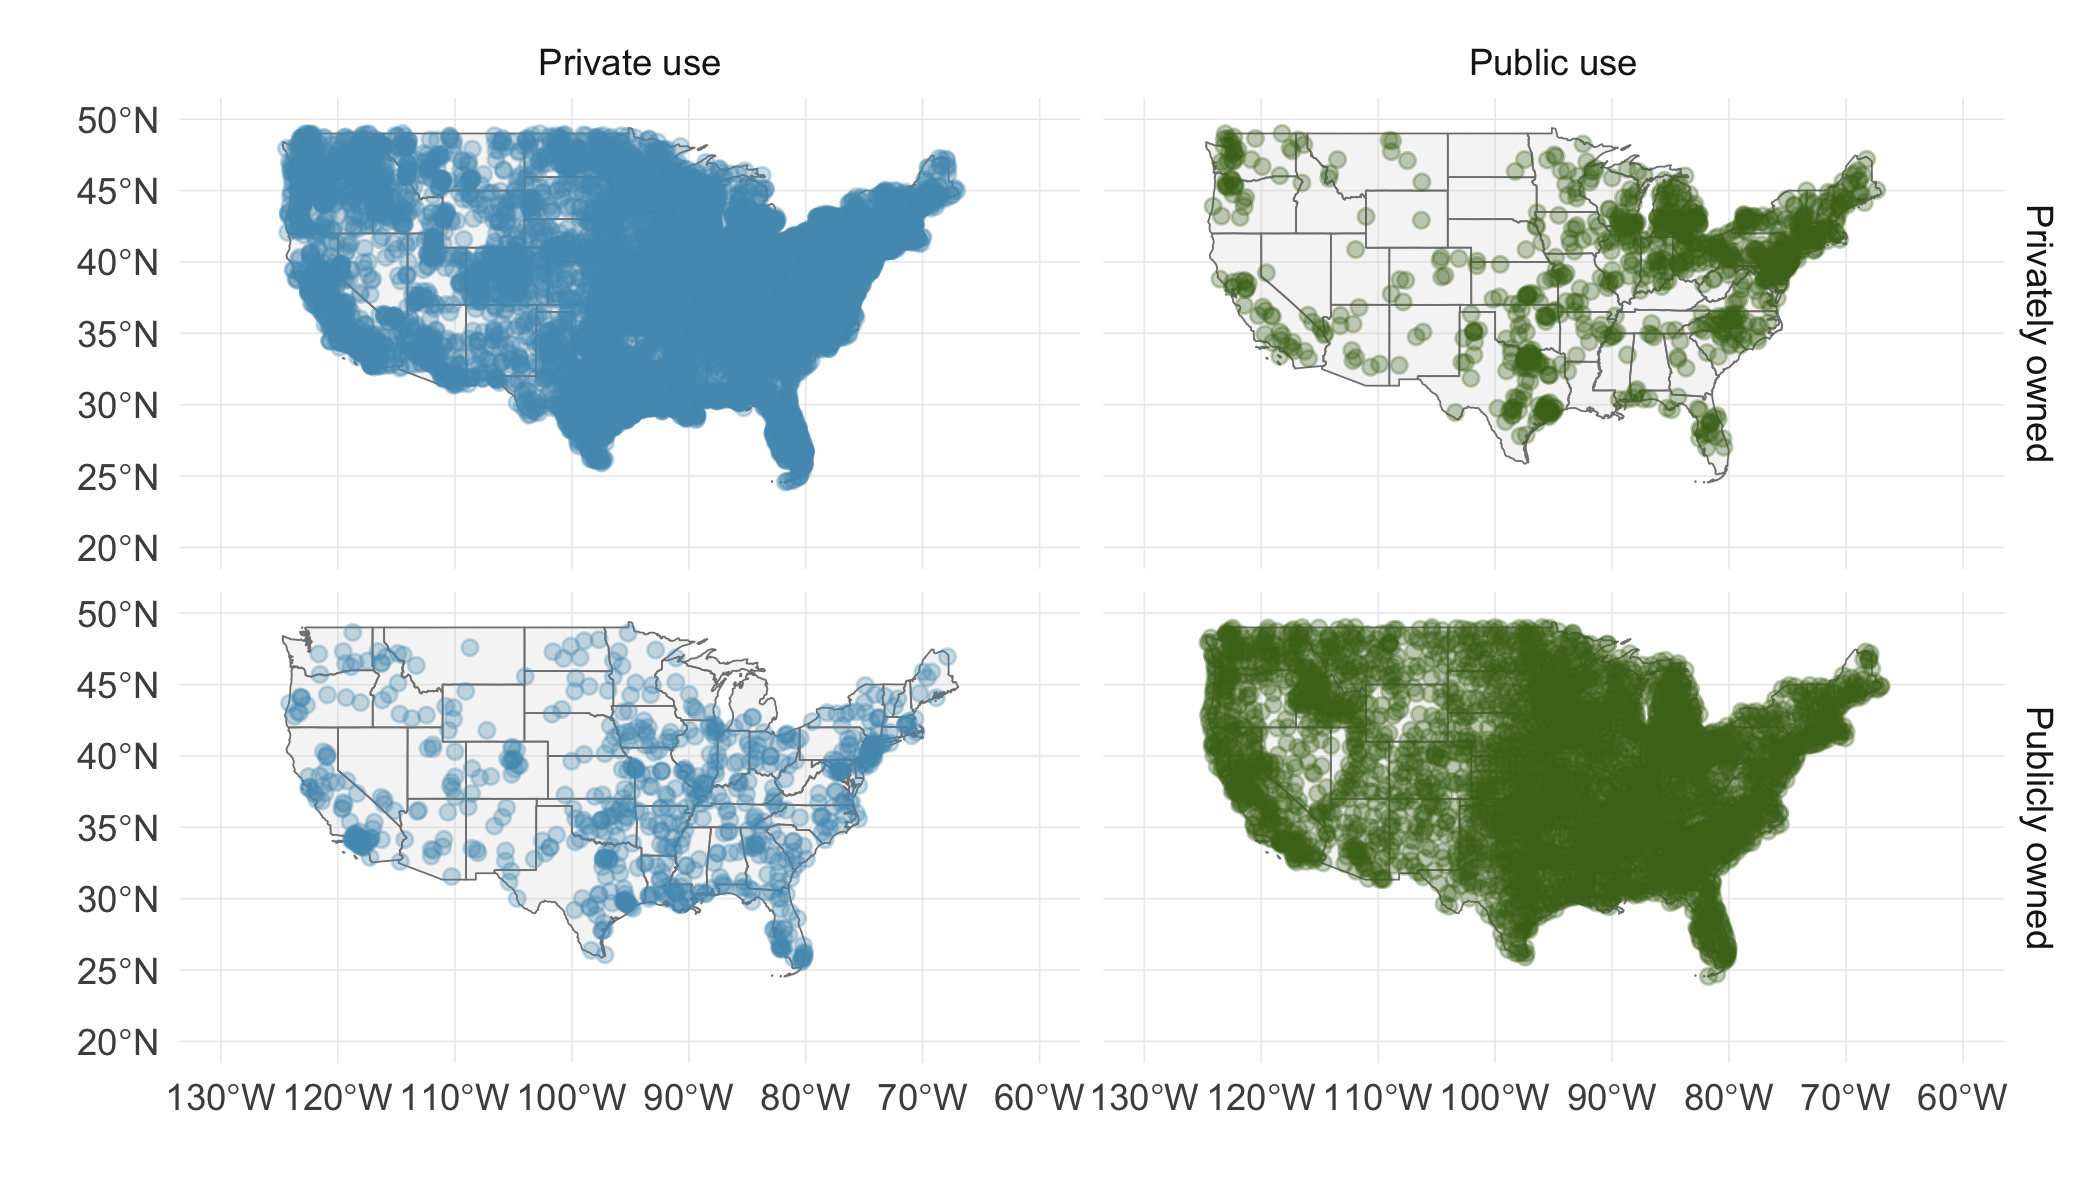
\includegraphics[width = 0.9\textwidth]{ch_intro_to_data/figures/eoce/airports/airports.png}
\end{center}
\begin{parts}
\item
    List the variables used in creating this visualization.
\item
    Indicate whether each variable in the study is numerical
    or categorical.
    If numerical, identify as continuous or discrete.
    If categorical, indicate if the variable is ordinal.
\end{parts}
}{}

% 12

\eoce{\qt{UN Votes\label{unvotes}}
The visualization below shows voting patterns in 
the United States, Canada, and Mexico in the United Nations General Assembly 
on a variety of issues. Specifically, for a given year between 1946 and 2015, 
it displays the percentage of roll calls in which the country voted yes for 
each issue. This visualization was constructed based on a dataset where each 
observation is a country/year pair.\footfullcite{data:unvotes}
\begin{center}
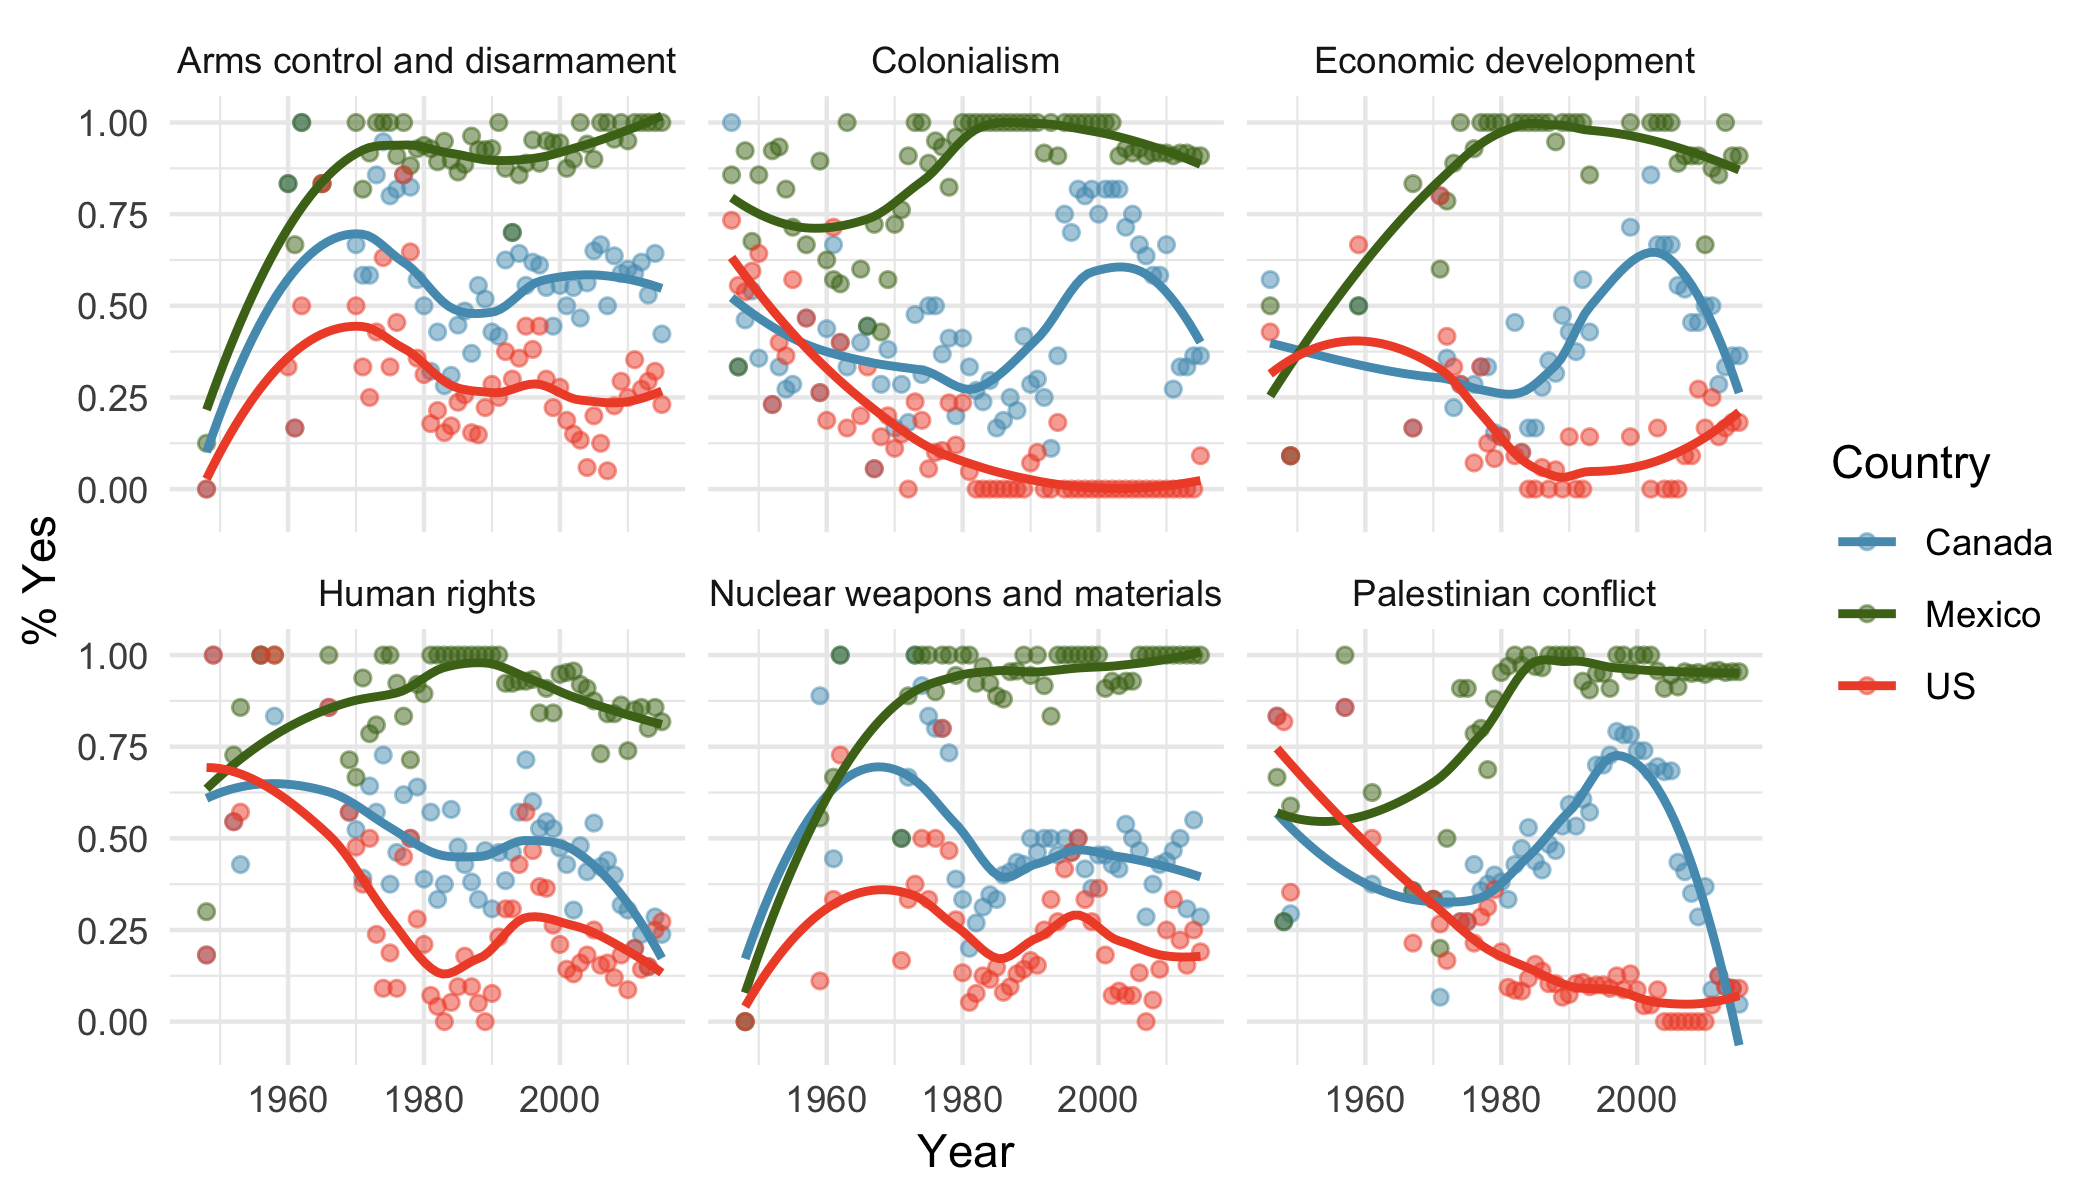
\includegraphics[width = 0.9\textwidth]{ch_intro_to_data/figures/eoce/unvotes/unvotes.png}
\end{center}
\begin{parts}
\item List the variables used in creating this visualization.
\item Indicate whether each variable in the study is numerical or categorical. 
If numerical, identify as continuous or discrete. If categorical, indicate if 
the variable is ordinal.
\end{parts}
}{}
}




%%%%%
\section{Sampling principles and strategies}
\label{overviewOfDataCollectionPrinciples}
\label{section_obs_data_sampling}

\index{sample|(}
\index{population|(}

The first step in conducting research is to identify topics
or questions that are to be investigated.
A clearly laid out research question is helpful in identifying
what subjects or cases should be studied and what variables are
important.
It is also important to consider \emph{how} data are collected
so that they are reliable and help achieve the research goals.


\subsection{Populations and samples}
\label{populationsAndSamples}

\noindent%
Consider the following three research questions:
\begin{enumerate}
\setlength{\itemsep}{0mm}
\item
    What is the average mercury content in swordfish
    in the Atlantic Ocean?
\item
    \label{timeToGraduationQuestionForUCLAStudents}%
    Over the last 5 years, what is the average time
    to complete a degree for Duke undergrads?
\item
    \label{identifyPopulationOfStentStudy}%
    Does a new drug reduce the number of deaths in patients
    with severe heart disease?
\end{enumerate}
Each research question refers to a target \term{population}. In the first question, the target population is all swordfish in the Atlantic ocean, and each fish represents a case. Often times, it is too expensive to collect data for every case in a population. Instead, a sample is taken. A \term{sample} represents a subset of the cases and is often a small fraction of the population. For instance, 60 swordfish (or some other number) in the population might be selected, and this sample data may be used to provide an estimate of the population average and answer the research question.

\begin{exercisewrap}
\begin{nexercise}\label{identifyingThePopulationForTwoQuestionsInPopAndSampSubsection}%
For the second and third questions above,
identify the target population and what
represents an individual case.\footnotemark
\end{nexercise}
\end{exercisewrap}
\footnotetext{(\ref{timeToGraduationQuestionForUCLAStudents})
    The first question is only relevant
    to students who complete their degree;
    the average cannot be computed using a student
    who never finished her degree.
    Thus, only Duke undergrads who
    graduated in the last five years represent cases
    in the population under consideration.
    Each such student is an individual case.
    (\ref{identifyPopulationOfStentStudy})~A person with
    severe heart disease represents a case.
    The population includes all people with severe heart
    disease.}


\subsection{Anecdotal evidence}
\label{anecdotalEvidenceSubsection}

\index{bias|(}

\noindent%
Consider the following possible responses to the three research questions:
\begin{enumerate}
\setlength{\itemsep}{0mm}
\item
    A man on the news got mercury poisoning from eating swordfish,
    so the average mercury concentration in swordfish must be
    dangerously high.
\item\label{iKnowThreeStudentsWhoTookMoreThan7YearsToGraduateAtDuke}
    I met two students who took more than 7 years to graduate
    from Duke, so it must take longer to graduate at Duke than
    at many other colleges.
\item\label{myFriendsDadDiedAfterSulphinpyrazon}
    My friend's dad had a heart attack and died after they gave
    him a new heart disease drug, so~the drug must not work.
\end{enumerate}
Each conclusion is based on data.
However, there are two problems.
First, the data only represent one or two cases.
Second, and more importantly, it is unclear whether these cases
are actually representative of the population.
Data collected in this haphazard fashion are called
\term{anecdotal evidence}.

\setlength{\captionwidth}{\textwidth-75mm}
\begin{figure}[h]
  \centering
  \hspace{8mm}\Figuress{55mm}{mnWinter}{mnWinter}\hspace{4mm}
  \begin{minipage}[b]{\textwidth-75mm}
    \caption[anecdotal evidence]{In February 2010,
        some media pundits cited one large snow storm
        as valid evidence against global warming.
        As comedian Jon Stewart pointed out,
        ``It's one storm, in one region, of one country.''
    \label{mnWinter}}
  \end{minipage}
\end{figure}
\setlength{\captionwidth}{\mycaptionwidth}

\begin{onebox}{Anecdotal evidence}
Be careful of data collected in a haphazard fashion.
Such evidence may be true and verifiable, but it may
only represent extraordinary cases.
\end{onebox}

\D{\newpage}

Anecdotal evidence typically is composed of unusual cases that we recall based on their striking characteristics. For instance, we are more likely to remember the two people we met who took 7~years to graduate than the six others who graduated in four years. Instead of looking at the most unusual cases, we should examine a sample of many cases that represent the population.

\subsection{Sampling from a population}

\index{sample!random sample|(}
\index{sample!bias|(}

We might try to estimate the time to graduation for Duke
undergraduates in the last 5 years by collecting a sample
of students.
All graduates in the last 5 years represent the
\emph{population}\index{population}, and graduates who are
selected for review are collectively called the
\emph{sample}\index{sample}.
In general, we always seek to \emph{randomly} select a sample
from a population.
The most basic type of random selection is equivalent to how
raffles are conducted.
For example, in selecting graduates, we could write each
graduate's name on a raffle ticket and draw 100 tickets.
The selected names would represent a random sample of 100 graduates.
We pick samples randomly to reduce the chance we introduce biases.

\begin{figure}[ht]
  \centering
  \Figures{0.5}{popToSample}{popToSampleGraduates}
  \caption{In this graphic, five graduates are randomly
      selected from the population to be included in the
      sample.}
  \label{popToSampleGraduates}
\end{figure}

\begin{examplewrap}
\begin{nexample}{Suppose we ask a student who happens to be
    majoring in nutrition to select several graduates for
    the study.
    What kind of students do you think she might collect?
    Do you think her sample would be representative of all
    graduates?}
  Perhaps she would pick a disproportionate number of graduates
  from health-related fields.
  Or~perhaps her selection would be a good representation
  of the population.
  When selecting samples by hand, we run the risk of picking
  a \termsub{biased}{sample!bias} sample, even if their bias
  isn't intended.
\end{nexample}
\end{examplewrap}

\begin{figure}
  \centering
  \Figures{0.5}{popToSample}{popToSubSampleGraduates}
  \caption{Asked to pick a sample of graduates,
      a nutrition major might inadvertently pick a
      disproportionate number of graduates from
      health-related majors.}
  \label{popToSubSampleGraduates}
\end{figure}

\D{\newpage}

If someone was permitted to pick and choose exactly which
graduates were included in the sample, it is entirely possible
that the sample could be skewed to that person's interests,
which may be entirely unintentional.
This introduces \term{bias} into a sample.
Sampling randomly helps resolve this problem.
The most basic random sample is called a
\term{simple random sample}, and which is equivalent to using
a raffle to select cases.
This means that each case in the population has an equal chance
of being included and there is no implied connection between
the cases in the sample.

The act of taking a simple random sample helps minimize bias.
However, bias can crop up in other ways.
Even when people are picked at random, e.g. for surveys,
caution must be exercised if the
\term{non-response rate}
\index{sample!non-response rate|textbf} is high.
For instance, if only 30\% of the people randomly sampled
for a survey actually respond, then it is unclear whether
the results are \term{representative} of the entire population.
This \term{non-response bias}
\index{sample!non-response bias|textbf} can skew results.

\begin{figure}[h]
  \centering
  \Figures{0.5}{popToSample}{surveySample}
  \caption{Due to the possibility of non-response,
      surveys studies may only reach a certain group
      within the population.
      It is difficult, and often times impossible,
      to completely fix this problem.}
  \label{surveySample}
\end{figure}

Another common downfall is a
\term{convenience sample}\index{sample!convenience sample},
where individuals who are easily accessible are more likely
to be included in the sample.
For instance, if a political survey is done by stopping people
walking in the Bronx, this will not represent all of New York City.
It is often difficult to discern what sub-population a convenience
sample represents.

\begin{exercisewrap}
\begin{nexercise}
We can easily access ratings for products, sellers, and companies through websites. These ratings are based only on those people who go out of their way to provide a rating. If 50\% of online reviews for a product are negative, do you think this means that 50\% of buyers are dissatisfied with the product?\footnotemark
\end{nexercise}
\end{exercisewrap}
\footnotetext{Answers will vary.
    From our own anecdotal experiences, we believe people
    tend to rant more about products that fell below
    expectations than rave about those that perform as
    expected.
    For this reason, we suspect there is a negative bias
    in product ratings on sites like Amazon.
    However, since our experiences may not be
    representative, we also keep an open mind.}

\index{sample!bias|)}
\index{sample!random sample|)}
\index{bias|)}
\index{population|)}
\index{sample|)}


\D{\newpage}

\subsection{Observational studies}

Data where no treatment has been explicitly applied
(or explicitly withheld) is called \term{observational data}.
For instance, the loan data and county data described in
Section~\ref{dataBasics}
are both examples of observational data.
%It is important to collect such data in
%a thoughtful and rigorous manner so that statistical
%analyses based on the data can have meaningful
%and generalizable results.
Making causal conclusions based on experiments is often reasonable.
However, making the same causal conclusions based on observational
data can be treacherous and is not recommended.
Thus, observational studies are generally only sufficient
to show associations or form hypotheses that we later check
using experiments.

\begin{exercisewrap}
\begin{nexercise}\label{sunscreenLurkingExample}%
Suppose an observational study tracked sunscreen use and skin cancer, and it was found that the more sunscreen someone used, the more likely the person was to have skin cancer. Does this mean sunscreen \emph{causes} skin cancer?\footnotemark
\end{nexercise}
\end{exercisewrap}
\footnotetext{No.
    See the paragraph following the exercise for
    an explanation.}

Some previous research tells us that using sunscreen actually reduces skin cancer risk, so maybe there is another variable that can explain this hypothetical association between sunscreen usage and skin cancer. One important piece of information that is absent is sun exposure. If someone is out in the sun all day, she is more likely to use sunscreen \emph{and} more likely to get skin cancer. Exposure to the sun is unaccounted for in the simple investigation.
\begin{center}
  \Figures{0.55}{variables}{sunCausesCancer}
\end{center}
% Some studies:
% http://www.sciencedirect.com/science/article/pii/S0140673698121682
% http://archderm.ama-assn.org/cgi/content/abstract/122/5/537
% Study with a similar scenario to that described here:
% http://onlinelibrary.wiley.com/doi/10.1002/ijc.22745/full

Sun exposure is what is called a \term{confounding variable},\footnote{Also called a \term{lurking variable}, \term{confounding factor}, or a \term{confounder}.} which is a variable that is correlated with both the explanatory and response variables. While one method to justify making causal conclusions from observational studies is to exhaust the search for confounding variables, there is no guarantee that all confounding variables can be examined or measured.

%In the same way, the \data{county} data set is an observational study with confounding variables, and its data cannot easily be used to make causal conclusions.

\begin{exercisewrap}
\begin{nexercise}
Figure~\ref{multiunitsVsOwnership} shows a negative association
between the homeownership rate and the percentage of multi-unit
structures in a county.
However, it is unreasonable to conclude that there is a causal
relationship between the two variables.
Suggest a variable that might explain the negative
relationship.\footnotemark
\end{nexercise}
\end{exercisewrap}
\footnotetext{Answers will vary.
    Population density may be important.
    If a county is very dense, then this may require
    a larger fraction of residents to live in
    multi-unit structures.
    Additionally, the high density may contribute
    to increases in property value, making
    homeownership infeasible for many residents.}

Observational studies come in two forms:
prospective and retrospective studies.
A \term{prospective study} identifies individuals
and collects information as events unfold.
For instance, medical researchers may identify and follow
a group of patients over many years to assess
the possible influences of behavior on cancer risk.
One example of such a study is The Nurses' Health Study,
started in 1976 and expanded in 1989.
This prospective study recruits registered nurses and then
collects data from them using questionnaires.
\termsub{Retrospective studies}{retrospective studies}
collect data after events have taken place,
e.g. researchers may review past events in medical records.
Some data sets may contain both prospectively- and
retrospectively-collected variables.


\subsection{Four sampling methods}
\label{fourSamplingMethods}
\label{threeSamplingMethods}

Almost all statistical methods are based on the notion of implied randomness. If observational data are not collected in a random framework from a population, these statistical methods -- the estimates and errors associated with the estimates -- are not reliable. Here we consider four random sampling techniques: simple, stratified, cluster, and multistage sampling. Figures~\ref{simple_stratified} and~\ref{cluster_multistage} provide graphical representations of these techniques.

\begin{figure}
\centering
\includegraphics[width=\textwidth]{ch_intro_to_data/figures/samplingMethodsFigure/simple_stratified}
\caption{Examples of simple random\index{sample!simple random sampling} and stratified sampling\index{sample!stratified sampling}. In the top panel, simple random sampling was used to randomly select the 18 cases. In the bottom panel, stratified sampling was used: cases were grouped into strata, then simple random sampling was employed within \mbox{each stratum}.}
\label{simple_stratified}
\end{figure}

\termsub{Simple random sampling}{sample!simple random sampling} is probably the most intuitive form of random sampling. Consider the salaries of Major League Baseball (MLB) players, where each player is a member of one of the league's 30 teams. To take a simple random sample of 120 baseball players and their salaries, we could write the names of that season's several hundreds of players onto slips of paper, drop the slips into a bucket, shake the bucket around until we are sure the names are all mixed up, then draw out slips until we have the sample of 120 players. In general, a sample is referred to as ``simple random'' if each case in the population has an equal chance of being included in the final sample \emph{and} knowing that a case is included in a sample does not provide useful information about which other cases are included.

\termsub{Stratified sampling}{sample!stratified sampling}
is a divide-and-conquer sampling strategy.
The population is divided into groups called
\term{strata}\index{sample!strata|textbf}.
The strata are chosen so that similar cases are grouped
together, then a second sampling method, usually simple
random sampling, is employed within each stratum.
In~the baseball salary example, the teams could represent
the strata, since some teams have a lot more money
(up to 4~times as much!).
Then we might randomly sample 4 players from each team for
a total of 120 players.

Stratified sampling is especially useful when the cases in each stratum are very similar with respect to the outcome of interest. The downside is that analyzing data from a stratified sample is a more complex task than analyzing data from a simple random sample. The analysis methods introduced in this book would need to be extended to analyze data collected using stratified sampling.

\begin{examplewrap}
\begin{nexample}{Why would it be good for cases within
    each stratum to be very similar?}
  We might get a more stable estimate for the subpopulation
  in a stratum if the cases are very similar,
  leading to more precise estimates within each group.
  When we combine these estimates into a single estimate
  for the full population, that population estimate will
  tend to be more precise since each individual group
  estimate is itself more precise.
\end{nexample}
\end{examplewrap}

In a \termsub{cluster sample}{sample!cluster sample}, we break up the population into many groups, called \termsub{clusters}{sample!cluster}. Then we sample a fixed number of clusters and include all observations from each of those clusters in the sample. A \termsub{multistage sample}{sample!multistage sample} is like a cluster sample, but rather than keeping all observations in each cluster, we collect a random sample within each selected cluster. %Multistage sampling is similar to stratified sampling in its process, except that stratified sampling requires observations be sampled from \emph{every} stratum.

\begin{figure}
  \centering
  \Figures{}{samplingMethodsFigure}{cluster_multistage}
  \caption{Examples of cluster\index{sample!cluster sampling}
  and multistage sampling\index{sample!multistage sampling}.
  In the top panel, cluster sampling was used:
  data were binned into nine clusters, three of these clusters
  were sampled, and all observations within these three cluster
  were included in the sample.
  In the bottom panel, multistage sampling was used,
  which differs from cluster sampling only in that we
  randomly select a subset of each cluster to be included
  in the sample rather than measuring every case in each
  sampled cluster.}
\label{cluster_multistage}
\end{figure}

Sometimes cluster or multistage sampling can be more economical
than the alternative sampling techniques.
Also, unlike stratified sampling, these approaches are most
helpful when there is a lot of case-to-case variability within
a cluster but the clusters themselves don't look very different
from one another.
For example, if neighborhoods represented clusters, then cluster
or multistage sampling work best when the neighborhoods are very
diverse.
A~downside of these methods is that more advanced techniques
are typically required to analyze the data, though the methods
in this book can be extended to handle such data.

\begin{examplewrap}
\begin{nexample}{Suppose we are interested in estimating
    the malaria rate in a densely tropical portion of rural
    Indonesia.
    We learn that there are 30 villages in that part of the
    Indonesian jungle, each more or less similar to the next.
    Our goal is to test 150 individuals for malaria.
    What sampling method should be employed?}
  A simple random sample would likely draw individuals from
  all 30 villages, which could make data collection extremely
  expensive.
  Stratified sampling would be a challenge since it is
  unclear how we would build strata of similar individuals.
  However, cluster sampling or multistage sampling seem like
  very good ideas.
  If we decided to use multistage sampling, we might randomly
  select half of the villages, then randomly select
  10 people from each.
  This would probably reduce our data collection costs
  substantially in comparison to a simple random sample,
  and the cluster sample would still give us reliable
  information, even if we would need to analyze the data
  with slightly more advanced methods than we discuss
  in this book.
\end{nexample}
\end{examplewrap}


{\exercisesheader{}

% 13

\eoce{\qt{Air pollution and birth outcomes, scope of inference\label{scope_airpoll}} 
Exercise~\ref{study_components_airpoll} introduces a study where researchers 
collected data to examine the relationship between air pollutants and preterm 
births in Southern California. During the study air pollution levels were 
measured by air quality monitoring stations. Length of gestation data were 
collected on 143,196 births between the years 1989 and 1993, and air pollution 
exposure during gestation was calculated for each birth.
\begin{parts}
\item Identify the population of interest and the sample in this study.
\item Comment on whether or not the results of the study can be generalized to the 
population, and if the findings of the study can be used to establish causal relationships.
\end{parts}
}{}

% 14

\eoce{\qt{Cheaters, scope of inference\label{scope_cheaters}} 
Exercise~\ref{study_components_cheaters} introduces a study where researchers 
studying the relationship between honesty, age, and self-control conducted an 
experiment on 160 children between the ages of 5 and 15. The researchers asked 
each child to toss a fair coin in private and to record the outcome (white or black) 
on a paper sheet, and said they would only reward children who report white. 
Half the students were explicitly told not to cheat and the others were not given 
any explicit instructions. Differences were observed in the cheating rates in the
instruction and no instruction groups, as well as some differences across 
children's characteristics within each group.
\begin{parts}
\item Identify the population of interest and the sample in this study.
\item Comment on whether or not the results of the study can be generalized to the 
population, and if the findings of the study can be used to establish causal 
relationships.
\end{parts}
}{}

% 15

\eoce{\qt{Buteyko method, scope of inference\label{scope_buteyko}} 
Exercise~\ref{study_components_buteyko} introduces a study on using the Buteyko 
shallow breathing technique to reduce asthma symptoms and improve quality of life.
As part of this study 600 asthma patients aged 18-69 who relied on medication for 
asthma treatment were recruited and randomly assigned to two groups: one practiced 
the Buteyko method and the other did not. Those in the Buteyko group experienced,
on average, a significant reduction in asthma symptoms and an improvement in quality 
of life.
\begin{parts}
\item Identify the population of interest and the sample in this study.
\item Comment on whether or not the results of the study can be generalized to the 
population, and if the findings of the study can be used to establish causal 
relationships.
\end{parts}
}{}

% 16

\eoce{\qt{Stealers, scope of inference\label{scope_stealers}} 
Exercise~\ref{study_components_stealers} introduces a study on the relationship 
between socio-economic class and unethical behavior. As part of this study 129 
University of California Berkeley undergraduates were asked to identify themselves 
as having low or high social-class by comparing themselves to others with the most 
(least) money, most (least) education, and most (least) respected jobs. They were 
also presented  with a jar of individually wrapped candies and informed that the
candies were for children in a nearby laboratory, but that they could take some if 
they wanted. After completing some unrelated tasks, participants reported the 
number of candies they had taken. It was found that those who were identified as 
upper-class took more candy than others.
\begin{parts}
\item Identify the population of interest and the sample in this study.
\item Comment on whether or not the results of the study can be generalized to the 
population, and if the findings of the study can be used to establish causal 
relationships.
\end{parts}
}{}

% 17

\eoce{\qt{Relaxing after work\label{relax_after_work_definitions}} The General 
Social Survey asked the question, ``After an average work day, about how many 
hours do you have to relax or pursue activities that you enjoy?" to a random 
sample of 1,155 Americans. The average relaxing time was found to be 1.65 
hours. Determine which of the following is an observation, a variable, a 
sample statistic (value calculated based on the observed sample), or a 
population parameter.
\begin{parts}
\item An American in the sample.
\item Number of hours spent relaxing after an average work day.
\item 1.65.
\item Average number of hours all Americans spend relaxing after an average 
work day.
\end{parts}
}{}

% 18

\eoce{\qt{Cats on YouTube\label{cats_on_youtube_definitions}} Suppose you want to 
estimate the percentage of videos on YouTube that are cat videos. It is 
impossible for you to watch all videos on YouTube so you use a random video 
picker to select 1000 videos for you. You find that 2\% of these videos are 
cat videos.Determine which of the following is an observation, a variable, 
a sample statistic (value calculated based on the observed sample), 
or a population parameter.
\begin{parts}
\item Percentage of all videos on YouTube that are cat videos.
\item 2\%.
\item A video in your sample.
\item Whether or not a video is a cat video.
\end{parts}
}{}

% 19

\eoce{\qt{Course satisfaction across sections\label{course_satisfaction_sections}} 
A large college class has 160 students. All 160 students attend the lectures 
together, but the students are divided into 4 groups, each of 40 students, 
for lab sections administered by different teaching assistants. The professor 
wants to conduct a survey about how satisfied the students are with the course, 
and he believes that the lab section a student is in might affect the student's 
overall satisfaction with the course.
\begin{parts}
\item What type of study is this?
\item Suggest a sampling strategy for carrying out this study.
\end{parts}
}{}

% 20

\eoce{\qt{Housing proposal across dorms\label{housing_proposal_dorms}} On a large 
college campus first-year students and sophomores live in dorms located on 
the eastern part of the campus and juniors and seniors live in dorms located 
on the western part of the campus. Suppose you want to collect student opinions 
on a new housing structure the college administration is proposing and you want 
to make sure your survey equally represents opinions from students from all years.
\begin{parts}
\item What type of study is this?
\item Suggest a sampling strategy for carrying out this study.
\end{parts}
}{}

% 21

\eoce{\qt{Internet use and life expectancy\label{internet_life_expectancy}} The 
following scatterplot was created as part of a study evaluating the 
relationship between estimated life expectancy at birth (as of 2014) and 
percentage of internet users (as of 2009) in 208 countries for which such 
data were available.\footfullcite{data:ciaFactbook}

\noindent\begin{minipage}[c]{0.44\textwidth}
\begin{parts}
\item Describe the relationship between life expectancy and percentage of 
internet users.
\item What type of study is this?
\item State a possible confounding variable that might explain this relationship 
and describe its potential effect.
\end{parts} \vspace{15mm}
\end{minipage}
\begin{minipage}[r]{0.55\textwidth}
\hfill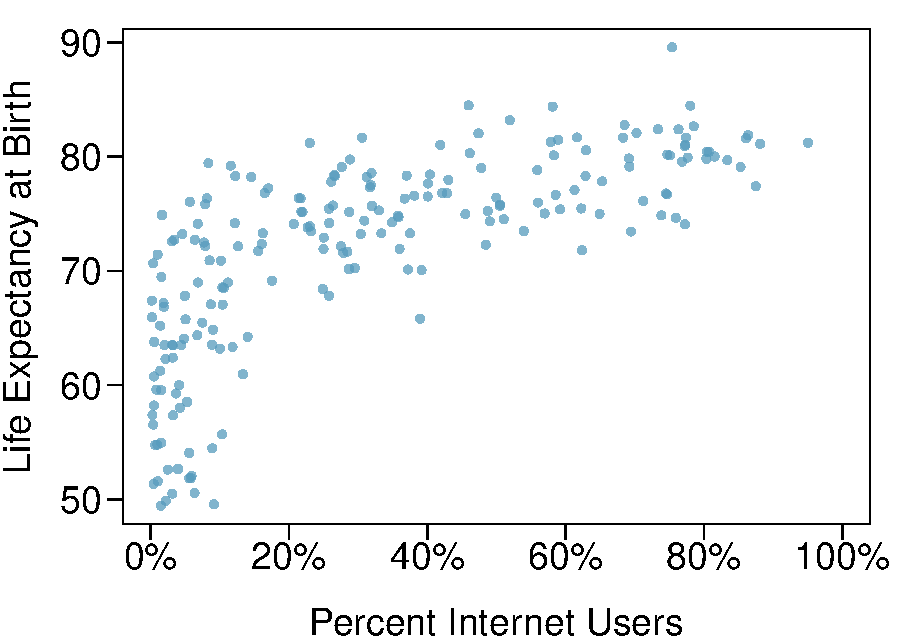
\includegraphics[width = 0.87\textwidth]{ch_intro_to_data/figures/eoce/internet_life_expectancy/internet_life_expectancy}
\end{minipage}
}{}

% 22

\eoce{\qt{Stressed out, Part I\label{stressed_out_observational}} A study that 
surveyed a random sample of otherwise healthy high school students found that 
they are more likely to get muscle cramps when they are stressed. The study 
also noted that students drink more coffee and sleep less when they are 
stressed.
\begin{parts}
\item What type of study is this?
\item Can this study be used to conclude a causal relationship between 
increased stress and muscle cramps?
\item State possible confounding variables that might explain the observed 
relationship between increased stress and muscle cramps. 
\end{parts}
}{}

% 23

\eoce{\qt{Evaluate sampling methods\label{evaluate_sampling_methods}} A university wants to 
determine what fraction of its undergraduate student body support a new \$25 annual fee 
to improve the student union. For each proposed method below, indicate whether 
the method is reasonable or not.
\begin{parts}
\item Survey a simple random sample of 500 students.
\item Stratify students by their field of study, then sample 10\% of students from  
each stratum.
\item Cluster students by their ages (e.g. 18 years old in one cluster, 19 years 
old in one cluster, etc.), then randomly sample three clusters and survey all 
students in those clusters.
\end{parts}
}{}

% 24

\eoce{\qt{Random digit dialing\label{random_digit_dialing}} The Gallup Poll uses a 
procedure called random digit dialing, which creates phone numbers based on 
a list of all area codes in America in conjunction with the associated number 
of residential households in each area code. Give a possible reason the Gallup 
Poll chooses to use random digit dialing instead of picking phone numbers 
from the phone book.
}{}

% 25

\eoce{\qt{Haters are gonna hate, study confirms\label{scope_haters}}
A study published in the
\textit{Journal of Personality and Social Psychology}
asked a group of 200 randomly sampled men and
women to evaluate how they felt about various subjects,
such as camping, health care, architecture, taxidermy, 
crossword puzzles, and Japan in order to measure their
attitude towards mostly independent stimuli.
Then, they presented the participants with information
about a new product: a microwave oven. This microwave oven
does not exist, but the participants didn't know this,
and were given three positive and three negative fake reviews.
People who reacted positively to the subjects on the
dispositional attitude measurement also tended to react 
positively to the microwave oven, and those who reacted
negatively tended to react negatively to it.
Researchers concluded that ``some people tend to 
like things, whereas others tend to dislike things, and a more thorough 
understanding of this tendency will lead to a more thorough understanding of 
the psychology of attitudes." \footfullcite{Hepler:2013}
\begin{parts}
\item What are the cases?
\item What is (are) the response variable(s) in this study?
\item What is (are) the explanatory variable(s) in this study?
\item Does the study employ random sampling?
\item Is this an observational study or an experiment? Explain your reasoning.
\item Can we establish a causal link between the explanatory and response 
variables?
\item Can the results of the study be generalized to the population at large?
\end{parts}
}{}

% 26

\eoce{\qt{Family size\label{family_size}} Suppose we want to estimate household 
size, where a ``household" is defined as people living together in the 
same dwelling, and sharing living accommodations. If we select students 
at random at an elementary school and ask them what their family size is, 
will this be a good measure of household size? Or will our average be 
biased? If so, will it overestimate or underestimate the true value?
}{}

% 27

\eoce{\qt{Sampling strategies\label{sampling_strategies}} A statistics student who is curious about the relationship between the amount of time students spend on social networking sites and their performance at school decides to conduct a survey. Various research strategies for collecting data are described below. In each, name the sampling method proposed and any bias you might expect.
\begin{parts}
\item He randomly samples 40 students from the study's population, gives them the survey, asks them to fill it out and bring it back the next day.
\item He gives out the survey only to his friends, making sure each one of them fills out the survey.
\item He posts a link to an online survey on Facebook and asks his friends to fill out the survey.
\item He randomly samples 5 classes and asks a random sample of students from those classes to fill out the survey.
\end{parts}
}{}

% 28

\eoce{\qt{Reading the paper\label{reading_paper}} Below are excerpts from two 
articles published in the \emph{NY Times}:
\begin{parts}
\item An article titled \emph{Risks: Smokers Found More Prone to Dementia} 
states the following: \footfullcite{news:smokingDementia}
\begin{adjustwidth}{1em}{1em}
{\footnotesize ``Researchers analyzed data from 23,123 health plan members who 
participated in a voluntary exam and health behavior survey from 1978 to 1985, 
when they were 50-60 years old. 23 years later, about 25\% of the group had 
dementia, including 1,136 with Alzheimer's disease and 416 with vascular 
dementia. After adjusting for other factors, the researchers concluded that 
pack-a-day smokers were 37\% more likely than nonsmokers to develop dementia, 
and the risks went up with increased smoking; 44\% for one to two packs a day; 
and twice the risk for more than two packs."}
\end{adjustwidth}
Based on this study, can we conclude that smoking causes dementia later in 
life? Explain your reasoning.
\item Another article titled \emph{The School Bully Is Sleepy} states the 
following: \footfullcite{news:bullySleep}
\begin{adjustwidth}{1em}{1em}
{\footnotesize ``The University of Michigan study, collected survey data from 
parents on each child's sleep habits and asked both parents and teachers to 
assess behavioral concerns. About a third of the students studied were 
identified by parents or teachers as having problems with disruptive behavior 
or bullying. The researchers found that children who had behavioral issues and 
those who were identified as bullies were twice as likely to have shown 
symptoms of sleep disorders."}
\end{adjustwidth}
A friend of yours who read the article says, ``The study shows that sleep 
disorders lead to bullying in school children." Is this statement justified? 
If not, how best can you describe the conclusion that can be drawn from this 
study?
\end{parts}
}{}
}






%%%%%
\section{Experiments}
\label{experimentsSection}

%\sectionintro{
Studies where the researchers assign treatments to cases are called \termsub{experiments}{experiment}. When this assignment includes randomization, e.g.~using a coin flip to decide which treatment a patient receives, it is called a \term{randomized experiment}. Randomized experiments are fundamentally important when trying to show a causal connection between two variables.
%}\setstretch{1.0}


\subsection{Principles of experimental design}
\label{experimentalDesignPrinciples}

\noindent{}Randomized experiments are generally built on four principles.

\begin{description}
\item[Controlling.]
    Researchers assign treatments to cases, and they do their
    best to \term{control} any other differences in the
    groups.\footnote{This is a different concept than
      a \emph{control group}, which we discuss in
      the second principle and in
      Section~\ref{biasInHumanExperiments}.}
    For example, when patients take a drug in pill form,
    some patients take the pill with only a sip of water
    while others may have it with an entire glass of water.
    To control for the effect of water consumption,
    a doctor may ask all patients to drink a 12 ounce glass
    of water with the pill.
\item[Randomization.] Researchers randomize patients into treatment groups to account for variables that cannot be controlled. For example, some patients may be more susceptible to a disease than others due to their dietary habits. Randomizing patients into the treatment or control group helps even out such differences, and it also prevents accidental bias from entering the study.
\item[Replication.] The more cases researchers observe, the more accurately they can estimate the effect of the explanatory variable on the response. In a single study, we \term{replicate} by collecting a sufficiently large sample. Additionally, a group of scientists may replicate an entire study to verify an earlier finding.

\begin{figure}
  \centering
  \Figure{0.82}{figureShowingBlocking}
  \caption{Blocking using a variable depicting patient risk.
      Patients are first divided into low-risk and high-risk
      blocks, then each block is evenly separated into the
      treatment groups using randomization.
      This strategy ensures an equal representation of patients
      in each treatment group from both the low-risk and high-risk
      categories.}
  \label{figureShowingBlocking}
\end{figure}

\item[Blocking.] Researchers sometimes know or suspect that variables, other than the treatment, influence the response. Under these circumstances, they may first group individuals based on this variable into \term{blocks} and then randomize cases within each block to the treatment groups. This strategy is often referred to as \term{blocking}. For instance, if we are looking at the effect of a drug on heart attacks, we might first split patients in the study into low-risk and high-risk blocks, then randomly assign half the patients from each block to the control group and the other half to the treatment group, as shown in Figure~\ref{figureShowingBlocking}. This strategy ensures each treatment group has an equal number of low-risk and high-risk patients.
\end{description}

It is important to incorporate the first three experimental
design principles into any study, and this book describes
applicable methods for analyzing data from such experiments.
Blocking is a slightly more advanced technique, and statistical
methods in this book may be extended to analyze data collected
using blocking.

\subsection{Reducing bias in human experiments}
\label{biasInHumanExperiments}

Randomized experiments are the gold standard for data collection,
but they do not ensure an unbiased perspective into the cause and
effect relationship in all cases.
Human studies are perfect examples where bias can unintentionally
arise.
Here we reconsider a study where a new drug was used to treat
heart attack patients.
In particular, researchers wanted to know if the drug reduced
deaths in patients.

These researchers designed a randomized experiment because they wanted to draw causal conclusions about the drug's effect. Study volunteers\footnote{Human subjects are often called \term{patients}, \term{volunteers}, or \term{study participants}.} were randomly placed into two study groups. One group, the \term{treatment group}, received the drug. The other group, called the \term{control group}, did not receive any drug treatment.

Put yourself in the place of a person in the study. If you are in the treatment group, you are given a fancy new drug that you anticipate will help you. On the other hand, a person in the other group doesn't receive the drug and sits idly, hoping her participation doesn't increase her risk of death. These perspectives suggest there are actually two effects: the one of interest is the effectiveness of the drug, and the second is an emotional effect that is difficult to quantify.

Researchers aren't usually interested in the emotional effect,
which might bias the study.
To circumvent this problem, researchers do not want patients
to know which group they are in.
When researchers keep the patients uninformed about their
treatment, the study is said to be \term{blind}.
But there is one problem:
if a patient doesn't receive a treatment, she will know she
is in the control group.
The solution to this problem is to give fake treatments to
patients in the control group.
A fake treatment is called a \term{placebo}, and an effective
placebo is the key to making a study truly blind.
A classic example of a placebo is a sugar pill that is made
to look like the actual treatment pill.
Often times, a placebo results in a slight but real
improvement in patients.
This effect has been dubbed the \term{placebo~effect}.

The patients are not the only ones who should be blinded:
doctors and researchers can accidentally bias a study.
When a doctor knows a patient has been given the real treatment,
she might inadvertently give that patient more attention or care
than a patient that she knows is on the placebo.
To guard against this bias, which again has been found to have
a measurable effect in some instances, most modern studies employ
a \term{double-blind} setup where doctors or researchers who
interact with patients are, just like the patients,
unaware of who is or is not receiving the
treatment.\footnote{There are always some researchers involved
  in the study who do know which patients are receiving which
  treatment.
  However, they do not interact with the study's patients and
  do not tell the blinded health care professionals who is
  receiving which treatment.}

\begin{exercisewrap}
\begin{nexercise}
Look back to the study in Section~\ref{basicExampleOfStentsAndStrokes} where researchers were testing whether stents were effective at reducing strokes in at-risk patients. Is this an experiment? Was the study blinded? Was it double-blinded?\footnotemark{}
\end{nexercise}
\end{exercisewrap}
\footnotetext{The researchers assigned the patients into their treatment groups, so this study was an experiment. However, the patients could distinguish what treatment they received, so this study was not blind. The study could not be double-blind since it was not blind.}

\begin{exercisewrap}
\begin{nexercise}
\label{gp_sham_surgery}%
For the study in Section~\ref{basicExampleOfStentsAndStrokes},
could the researchers have employed a placebo?
If so, what would that placebo have looked like?\footnotemark{}
\end{nexercise}
\end{exercisewrap}
\footnotetext{Ultimately, can we make patients think they
  got treated from a surgery?
  In fact, we can, and some experiments use
  what's called a \term{sham surgery}.
  In a sham surgery, the patient does undergo surgery,
  but the patient does not receive the full treatment,
  though they will still get a placebo effect.}

You may have many questions about the ethics of
sham surgeries to create a placebo after reading
Guided Practice~\ref{gp_sham_surgery}.
These questions may have even arisen in your mind when
in the general experiment context, where a possibly
helpful treatment was withheld from individuals in the
control group;
the main difference is that a sham surgery tends to
create additional risk, while withholding a treatment
only maintains a person's risk.

There are always multiple viewpoints of experiments
and placebos, and rarely is it obvious which is
ethically ``correct''.
For instance, is it ethical to use a sham surgery
when it creates a risk to the patient?
However, if we don't use sham surgeries,
we may promote the use of a costly treatment that
has no real effect;
if this happens, money and other resources will be diverted
away from other treatments that are known to be helpful.
Ultimately, this is a difficult situation where
we cannot perfectly protect both the patients
who have volunteered for the study and the patients who
may benefit (or not) from the treatment in the future.


{


%_______________
\newpage\subsection*{Exercises} % Experiments

% 1

\eoce{\qt{Light and exam performance\label{light_exam_performance}} A study is designed to 
test the effect of light level on exam performance of students. The researcher believes 
that light levels might have different effects on males and females, so wants to make 
sure both are equally represented in each treatment. The treatments are fluorescent 
overhead lighting, yellow overhead lighting, no overhead lighting (only desk lamps). 
\begin{parts}
\item What is the response variable?
\item What is the explanatory variable? What are its levels?
\item What is the blocking variable? What are its levels?
\end{parts}
}{}

% 2

\eoce{\qt{Vitamin supplements\label{vitamin_supplement}} In order to assess the effectiveness 
of taking large doses of vitamin C in reducing the duration of the common cold, 
researchers recruited 400 healthy volunteers from staff and students at a university. A 
quarter of the patients were assigned a placebo, and the rest were evenly divided 
between 1g Vitamin C,  3g Vitamin C, or 3g Vitamin C plus additives to be taken at onset 
of a cold for the following two days. All tablets had identical appearance and packaging.
The nurses who handed the prescribed pills to the patients knew which patient received 
which treatment, but the researchers assessing the patients when they were sick did not. 
No significant differences were observed in any measure of cold duration or severity 
between the four medication groups, and the placebo group had the shortest duration of 
symptoms.\footfullcite{Audera:2001}
\begin{parts}
\item Was this an experiment or an observational study? Why?
\item What are the explanatory and response variables in this study?
\item Were the patients blinded to their treatment?
\item Was this study double-blind?
\item Participants are ultimately able to choose whether or not to use the pills 
prescribed to them. We might expect that not all of them will adhere and take their 
pills. Does this introduce a confounding variable to the study? Explain your reasoning.
\end{parts}
}{}

% 3

\eoce{\qt{Light, noise, and exam performance\label{light_noise_exam_performance}} A study is 
designed to test the effect of light level and noise level on exam performance of 
students. The researcher believes that light and noise levels might have different 
effects on males and females, so wants to make sure both are equally represented in each 
treatment. The light treatments considered are fluorescent overhead lighting, yellow 
overhead lighting, no overhead lighting (only desk lamps). The noise treatments 
considered are no noise,  construction noise, and human chatter noise.
\begin{parts}
\item What type of study is this?
\item How many factors are considered in this study? Identify them, and describe their 
levels.
\item What is the role of the sex variable in this study?
\end{parts}
}{}

% 4

\eoce{\qt{Music and learning\label{music_learning}} You would like to conduct an experiment in 
class to see if students learn better if they study without any music, with music that 
has no lyrics (instrumental), or with music that has lyrics. Briefly outline a design for 
this study.
}{}

% 5

\eoce{\qt{Soda preference\label{soda_preference}} You would like to conduct an experiment in 
class to see if your classmates prefer the taste of regular Coke or Diet Coke. Briefly 
outline a design for this study.
}{}

% 6

\eoce{\qt{Exercise and mental health\label{exercise_mental_health}} A researcher is interested 
in the effects of exercise on mental health and he proposes the following study: Use 
stratified random sampling to ensure representative proportions of 18-30, 31-40 and 41-
55 year olds from the population. Next, randomly assign half the subjects from each age 
group to exercise twice a week, and instruct the rest not to exercise. Conduct a mental 
health exam at the beginning and at the end of the study, and compare the results.
\begin{parts}
\item What type of study is this? 
\item What are the treatment and control groups in this study?
\item Does this study make use of blocking? If so, what is the blocking variable?
\item Does this study make use of blinding?
\item Comment on whether or not the results of the study can be used to establish a 
causal relationship between exercise and mental health, and indicate whether or not the 
conclusions can be generalized to the population at large.
\item Suppose you are given the task of determining if this proposed study should get 
funding. Would you have any reservations about the study proposal?
\end{parts}
}{}
}
